\ifdefined\XeTeXversion\else\pdfoutput=1\fi
\documentclass[10pt,twocolumn]{article}
\usepackage[letterpaper,margin=0.72in,columnsep=0.27in]{geometry}
\usepackage[T1]{fontenc}
\usepackage{amsmath,amssymb}
\usepackage{newtxtext,newtxmath}
\usepackage{booktabs,graphicx,microtype,url,array,enumitem,tikz,placeins,balance,float}
\usetikzlibrary{arrows.meta,positioning}
\usepackage[hidelinks]{hyperref}
\hypersetup{pdftitle={Distributionally Robust Portfolio Choice under Stochastic Volatility: A Review and Reproducible Multi-Asset Study},pdfauthor={Sheehan Mathur}}
\setlength{\parindent}{1em}
\setlength{\textfloatsep}{11pt plus 2pt minus 2pt}
\setlength{\belowcaptionskip}{3pt}
\raggedbottom
\setcounter{dbltopnumber}{3}
\renewcommand{\dbltopfraction}{0.9}
\renewcommand{\textfraction}{0.08}
\setlist{nosep,leftmargin=*}
\newcommand{\E}{\mathbb{E}}
\newcommand{\R}{\mathbb{R}}
\newcommand{\CVaR}{\operatorname{CVaR}}
\newcommand{\W}{\mathcal{W}}
\title{\bfseries Distributionally Robust Portfolio Choice under Stochastic Volatility\\[3pt]\Large A Review and Reproducible Multi-Asset Study}
\author{Sheehan Mathur\\[5pt]\normalsize Department of Computer Science and Engineering\\\normalsize Birla Institute of Technology and Science Pilani, Dubai Campus\\\normalsize\texttt{f20240212@dubai.bits-pilani.ac.in}}
\date{}
\begin{document}
\maketitle
\begin{center}\large\bfseries Abstract\end{center}
\noindent\textit{Distributionally robust optimization (DRO) addresses uncertainty about a return law in addition to risk under that law. This paper reviews established DRO methods and evaluates a reproducible portfolio pipeline without claiming a new optimization method. A persistence-anchored residual LSTM predicts changes in log rolling volatility. Physical Heston parameters are fitted annually to past returns using a latent-variance particle likelihood. A four-ETF mean-CVaR problem combines a Wasserstein penalty with quadratic risk. A preliminary single-asset analysis over 2019--2024 motivated the design, so that period is exploratory; 2025 supplies a separate retrospective confirmation period. Residual forecasting lowers RMSE against persistence by 16--21\% in exploration and 22--29\% in confirmation, although a simple rolling-window update remains competitive. Fitted Heston models have mixed predictive likelihood gains. A matched 20,000-scenario comparison under three independent seeds reduces Monte Carlo variation below the average robustness tilt, while robust-versus-nominal return differences remain statistically inconclusive. Strong 2025 performance is interpreted in light of a gold rally and concentrated gold holdings in a historical benchmark. A cash-enabled comparison separates asset composition from de-risking. The public release provides code, model records, aggregate results, and input hashes; numerical replication is conditional on access to matching provider inputs.}
\par\vspace{7pt}
\noindent\textbf{Keywords:} distributionally robust optimization; stochastic volatility; residual learning; Heston calibration; conditional value-at-risk; multi-asset portfolios.

\section{Introduction}
Portfolio decisions depend on an estimated distribution of future returns. Risk criteria summarize losses under that distribution, whereas distributionally robust optimization (DRO) evaluates specified perturbations of the distribution itself. A flexible volatility model and a conservative decision criterion address different parts of this problem. Combining them is therefore a modeling choice to validate, rather than evidence of improved investment performance.

\begin{figure}[t]
\centering
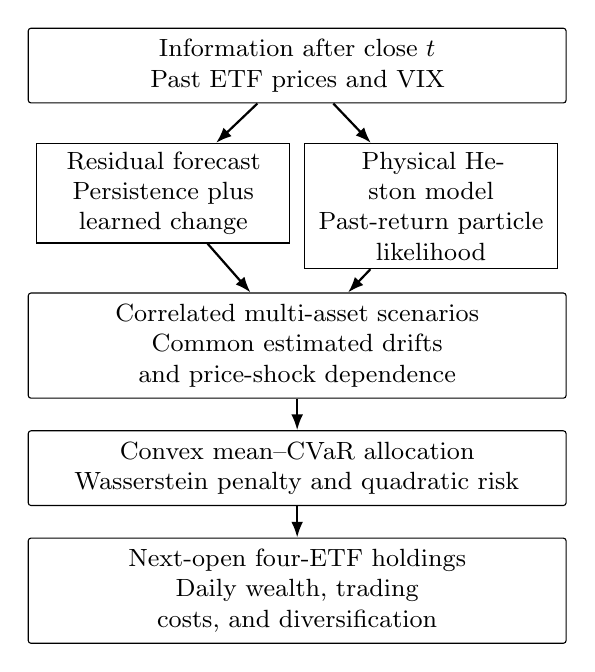
\begin{tikzpicture}[node distance=4mm,box/.style={draw,rounded corners=1pt,align=center,text width=6.55cm,inner sep=4pt,font=\small},half/.style={draw,align=center,text width=3.0cm,inner sep=3pt,font=\small},arr/.style={-{Latex[length=2mm]},thick}]
\node[box] (a) {Information after close $t$\\Past ETF prices and VIX};
\node[half,anchor=north] (b) at ([xshift=-17mm,yshift=-5mm]a.south) {Residual forecast\\Persistence plus\\learned change};
\node[half,anchor=north] (c) at ([xshift=17mm,yshift=-5mm]a.south) {Physical Heston model\\Past-return particle\\likelihood};
\node[box,below=24mm of a] (d) {Correlated multi-asset scenarios\\Common estimated drifts and price-shock dependence};
\node[box,below=of d] (e) {Convex mean--CVaR allocation\\Wasserstein penalty and quadratic risk};
\node[box,below=of e] (f) {Next-open four-ETF holdings\\Daily wealth, trading costs, and diversification};
\draw[arr] (a)--(b);\draw[arr] (a)--(c);\draw[arr] (b)--(d);\draw[arr] (c)--(d);\draw[arr] (d)--(e);\draw[arr] (e)--(f);
\end{tikzpicture}
\caption{The computational pipeline. Forecasting, parameter estimation, and optimization have separate benchmarks and diagnostics. The primary portfolio is fully invested, which holds gross exposure constant across model variants.}
\label{fig:pipeline}
\end{figure}

Mean--variance analysis organizes portfolio choices through expected returns and covariances \cite{markowitz}. Its formulation does not require normal returns, although those moments need not capture all downside preferences. CVaR makes tail losses explicit \cite{rockafellar}, while a Wasserstein ambiguity set specifies a geometry for changes in outcomes \cite{esfahani}. Stochastic-volatility dynamics describe time-varying dispersion; they do not eliminate distributional misspecification.

This paper develops a study project on these established components as a selective review and reproducible experiment. Three design choices are central. First, a neural forecast should demonstrate value beyond the persistence already present in its target. Second, stochastic-volatility parameters should be estimated from historically available data rather than treated as universal constants. Third, a portfolio experiment should distinguish diversification from a scalar switch between equity and cash.

We address these questions with a residual forecast, a fitted latent-variance model, and a four-asset convex allocation problem. The forecast includes an identity path, a zero-initialized correction head, and a validation-only shrinkage rule. The Heston likelihood conditions variance transitions on observed returns, retaining leverage. The allocation includes an explicit positive-definite quadratic risk term and uses a Euclidean transport metric, so robustness depends on the vector of weights. No per-asset cap forces diversification.

A preliminary single-asset analysis over 2019--2024 motivated the design, so that period is labeled exploratory. Economic coefficients were fixed before the multi-asset outcomes were inspected. A separately specified 2025 sample is a retrospective confirmation period, not a publicly preregistered prospective trial. Numerical accuracy is assessed through tighter likelihood searches and matched 20,000-scenario allocation runs under three independent seeds. Those checks do not select economic settings by future performance.

The main findings are qualified. Residual prediction substantially improves the neural comparison with persistence, but a mechanical rolling-window baseline explains much of the available target predictability. Estimated Heston parameters vary across assets and years, yet their predictive likelihood gains are mixed. Multi-asset allocations permit diversification at fixed exposure. A higher-scenario comparison reduces simulation variation, while incremental DRO return effects remain small and statistically uncertain. These findings support an educational synthesis rather than an algorithmic novelty or universal performance claim.

\section{Literature review}
\subsection{Risk and distributional ambiguity}
For a loss $L$ and confidence level $\alpha\in(0,1)$, the Rockafellar--Uryasev representation is
\begin{equation}
\CVaR_\alpha^P(L)=\inf_{\eta\in\R}\left\{\eta+\frac{\E_P[(L-\eta)_+]}{1-\alpha}\right\}.
\label{eq:cvar}
\end{equation}
For continuous laws, CVaR is the mean loss in the worst $1-\alpha$ fraction. Empirical distributions require consistent treatment of fractional mass at a quantile. Rounding a tail count arbitrarily can produce a different estimator.

Risk aversion under a specified law and ambiguity aversion over possible laws are distinct. A generic DRO problem is
\begin{equation}
\inf_{w\in\W}\sup_{Q\in\mathcal P}\E_Q[\ell(w,R)],
\end{equation}
where $\mathcal P$ represents the admissible distributional perturbations. A larger set strengthens the worst-case criterion and can sacrifice nominal performance. Whether this trade-off is useful depends on the set, loss, and data. Surveys and tutorials explain its connections to robust optimization, regularization, and statistical inference \cite{rahimian,kuhn,kuhntutorial}.

\subsection{Families of ambiguity sets}
\label{sec:families}
Moment-based sets constrain quantities such as means and covariances. Delage and Ye account for uncertainty in estimated moments and derive tractable formulations for important problem classes \cite{delage}. Such sets are useful when moment information is defensible, but results depend on the distributional freedom left by those restrictions.

Divergence-based sets bound a discrepancy from a nominal law. On finite scenario support, a $\phi$-divergence set takes the form
\begin{equation}
\mathcal P_\phi=\left\{q\in\Delta_N:\sum_i p_i\phi(q_i/p_i)\leq\delta\right\}.
\end{equation}
Ben-Tal et al. study uncertain probabilities and tractable robust counterparts for several choices \cite{bental}; Calafiore applies related discrete-distribution ambiguity to robust portfolio risk measures \cite{calafiore}, and Glasserman and Xu use relative-entropy neighborhoods to bound model risk \cite{glasserman}. In this representation, uncertainty reweights scenarios. It does not introduce a crash outcome missing from the selected support. Other divergence constructions can instead have continuous nominal distributions.

Optimal transport allows probability mass to move in the sample space at a cost. Under the absolute-value metric,
\begin{equation}
W_1(Q,P)=\inf_{\pi\in\Pi(Q,P)}\int |r-r'|\,\pi(dr,dr'),
\end{equation}
where $\Pi(Q,P)$ denotes couplings. A Wasserstein ball may therefore include outcomes outside an empirical support. Mohajerin Esfahani and Kuhn establish data-driven guarantees and convex reformulations \cite{esfahani}; Gao and Kleywegt derive strong duality for general transport costs \cite{gaokleywegt}; and Blanchet and Murthy develop a transport perspective on model risk \cite{blanchet}. A recurring theme is that Wasserstein robustness is equivalent, or close, to Lipschitz or variation regularization of the loss \cite{shafieezadeh,gaochen}. These results motivate the model below, subject to its support and sampling assumptions.

\begin{table}[t]
\centering\footnotesize\setlength{\tabcolsep}{3pt}
\caption{Ambiguity-set families used in portfolio DRO. Divergence refers to $\phi$-divergence sets on finite support. ``Support'' indicates whether worst-case laws may place mass on outcomes absent from the nominal law.}
\label{tab:families}
\begin{tabular}{@{}>{\raggedright}p{1.35cm}>{\raggedright}p{1.8cm}>{\raggedright}p{1.35cm}>{\raggedright\arraybackslash}p{2.50cm}@{}}\toprule
Family&Uncertain quantity&Support&Portfolio examples\\\midrule
Moment&Means, covariances&Any law matching moments&Delage and Ye \cite{delage}; worst-case CVaR \cite{zhu}\\
Divergence&Scenario probabilities&Nominal only&Ben-Tal et al.\ \cite{bental}; Calafiore \cite{calafiore}\\
Wasserstein&Outcome locations and probabilities&May extend beyond nominal&Pflug and Wozabal \cite{pflug}; Mohajerin Esfahani and Kuhn \cite{esfahani}; Blanchet et al.\ \cite{bcz}\\\bottomrule
\end{tabular}
\end{table}

No ambiguity family is uniformly preferable (Table~\ref{tab:families}). Moment sets express uncertainty about moments; finite-support divergence sets change scenario probabilities; transport sets impose a geometry on outcome changes. In particular, a radius of $0.001$ has different meaning for daily returns, monthly returns, or standardized features. Its units are part of the model.

\subsection{Financial applications and tail risk}
Worst-case CVaR portfolio optimization is well established. Zhu and Fukushima examine mixture, box, and ellipsoidal uncertainty, obtaining linear and second-order cone formulations \cite{zhu}. Pflug and Wozabal were among the first to use Kantorovich--Wasserstein balls for portfolio selection \cite{pflug}; Wasserstein mean-risk portfolios are studied in \cite{esfahani}; and Blanchet, Chen, and Zhou derive Wasserstein-robust mean--variance portfolios with a data-driven radius \cite{bcz}. Coupling a robust CVaR layer to a scenario generator therefore does not, by itself, constitute a new method.

Economic interpretation requires more than minimizing a risk statistic. A smaller drawdown may result from holding more cash, without better forecasting or timing. DeMiguel, Garlappi, and Uppal show that optimized portfolios often fail to beat naive $1/N$ allocation out of sample once estimation error is accounted for \cite{demiguel}. Comparisons should therefore disclose exposure and include simple allocations. A model can reduce expected shortfall while losing compound return or performing worse at similar exposure. The experiment explicitly examines these possibilities.

\subsection{Volatility and neural finance}
Heston dynamics describe a latent variance state; return--variance correlation affects asymmetry, while mean reversion controls variance persistence. The original option-pricing model uses a risk-neutral measure. Asset allocation needs a physical predictive law. Using a risk-neutral drift or treating an option calibration as a physical forecast requires additional justification. Rough-volatility evidence further suggests that a single Markovian variance factor is a simplification \cite{gatheral}.

LSTM networks learn temporal dependencies \cite{lstm}, but flexibility alone does not establish forecast value. Volatility forecasting has a long tradition of hard-to-beat simple models: Andersen and Bollerslev show that apparently poor forecasts often reflect noisy proxies \cite{andersenbollerslev}, and Hansen and Lunde find that parsimonious GARCH specifications are difficult to outperform in several settings \cite{hansenlunde}. Corsi's HAR-RV combines volatility components over different horizons \cite{corsi}, and neural networks trained on realized measures can improve on it \cite{bucci}. Persistence and parsimonious regressions are therefore necessary benchmarks. Our regression borrows the HAR structure for a rolling daily-return proxy, rather than reproducing the original intraday realized-variance estimator.

Other neural finance methods address different tasks. Deep hedging optimizes hedges under trading frictions \cite{buehler}, and arbitrage-free neural-SDE market models learn constrained option-market dynamics \cite{cohen}. These works provide context for learning with financial structure. Their findings do not validate the simpler state substitution studied here. The review is selective, guided by the experiment and representative surveys, rather than an exhaustive or systematic survey.


Recent comparative evidence also emphasizes horizon-specific econometric benchmarks rather than assuming that machine learning dominates \cite{kilic}. Estimation of physical-measure stochastic-volatility dynamics is a separate inference task: approximate likelihood and observable-moment approaches have their own sampling and proxy limitations \cite{azencott,azencottrealized}. Particle-filter approaches explicitly treat the variance as latent \cite{arulampalam,gruszka}. The present implementation uses these established ideas in a constrained numerical study.

\section{Forecasts and calibration}
\subsection{Information, target, and baselines}
Let $\mathcal F_t$ contain observations available after day $t$ closes. For daily log returns $r_t$, define the 21-day annualized volatility proxy and its next observation by
\begin{equation}
s_t=\sqrt{252}\operatorname{sd}_0(r_{t-20},\ldots,r_t),\qquad y_t=\log s_{t+1},
\end{equation}
where the standard deviation uses divisor 21. This is a rolling close-return proxy, not an intraday realized-volatility estimator. Adjacent windows share 20 observations. Consequently, persistence, $\widehat y_t=\log s_t$, is a demanding but necessary benchmark.

A further baseline accounts for the known observation leaving the window. Put $n=21$, $x=r_{t-20}$, $S=\sum_{j=0}^{20}r_{t-j}-x$, and $A=\sum_{j=0}^{20}r_{t-j}^2-x^2$. Let $m$ and $b$ be the current window's mean and mean square, interpreted as conditional estimates of $\E_t r_{t+1}$ and $\E_t r_{t+1}^2$. The expected updated population variance is
\begin{equation}
\widehat v^{\rm upd}_{t+1}=\frac{A+b}{n}-\frac{S^2+2Sm+b}{n^2}.
\label{eq:update}
\end{equation}
The window-update forecast is $\tfrac12\log(252\widehat v^{\rm upd}_{t+1})$, with a numerical positivity floor. Equation~\eqref{eq:update} is an elementary conditional-moment calculation. It tests whether an apparent neural improvement mainly recovers the window's mechanical update.

Other comparators are EWMA with decay 0.94 and a HAR-type OLS regression on the current log proxy and its 5- and 22-day averages. This regression borrows the horizon structure of HAR-RV \cite{corsi}; its data and estimator differ from intraday HAR-RV.

\subsection{Persistence-anchored residual LSTM}
The residual target and forecast are
\begin{align}
\Delta_t&=\log s_{t+1}-\log s_t,\\
\widehat y_t^{\rm res}&=\log s_t+g_y f_\varphi(X_{t-19:t}),\qquad
g_y\in\{0,\tfrac14,\tfrac12,\tfrac34,1\}.
\label{eq:residual}
\end{align}
The LSTM learns changes rather than reconstructing the volatility level. Its linear correction head starts at zero, so the initial network exactly reproduces persistence. That checkpoint remains eligible during early stopping. For each annual refit, the mean correction of three seeded networks is shrunk by $g_y$, chosen using the preceding validation year only.

Including $g_y=0$ guarantees that the selected ensemble's validation MSE is no larger than persistence MSE on those same validation observations. It does \emph{not} guarantee better test loss. Both the unshrunk residual ensemble and the selected forecast are reported, so the role of validation shrinkage remains visible.

The six input features are log return, log rolling volatility, the 20-day mean return, log VIX in decimal units, the outgoing return $r_{t-20}$, and its square. Including the outgoing observation gives the network access to information needed for \eqref{eq:update}. It is available at time $t$ and introduces no future return. A separate level LSTM uses the same features, sequence length, hidden dimension, optimizer, and chronological splits, but predicts $y_t$ directly. It is an ablation; the main neural comparison is the residual model against simple forecasts.

Each network has one 16-unit recurrent layer and a linear output, totaling 1,553 trainable parameters. We use Adam with learning rate $10^{-3}$, batch size 64, gradient clipping at norm 1, and at most 40 epochs. Six non-improving epochs trigger stopping. Seeds are 7, 17, and 27. Features are standardized on training data. Level targets use training mean and standard deviation; residual targets are scaled by their training standard deviation without mean centering, preserving the identity at zero output.

For test year $y$, training labels must be available before 1 January $y-1$. Labels observed during year $y-1$ supply validation. Splits use label availability dates, preventing the last training observation from using a future validation target. Previously observed evaluation outcomes may enter later annual fits once historically available.

\subsection{Physical Heston likelihood}
For asset $j$, the physical-measure dynamics are
\begin{align}
dS_{j,s}&=\mu_j S_{j,s}\,ds+\sqrt{v_{j,s}}S_{j,s}\,dW^S_{j,s},\\
dv_{j,s}&=\kappa_j(\theta_j-v_{j,s})\,ds+\xi_j\sqrt{v_{j,s}}\,dW^v_{j,s},\\
d\langle W^S_j,W^v_j\rangle_s&=\rho_j\,ds.
\end{align}
These are predictive physical parameters, not risk-neutral option parameters. Variance is latent. We do not estimate the CIR parameters by pretending that a smoothed rolling standard deviation is observed instantaneous variance.

Instead, a regularized daily Euler state-space model supplies an approximate likelihood. For $\delta=1/252$ and $v^+=\max(v,10^{-8})$,
\begin{align}
r_t\mid v_{t-1}&\sim N\bigl((\mu-\tfrac12v^+)\delta,v^+\delta\bigr),\\
z_t&=\frac{r_t-(\mu-\tfrac12v^+)\delta}{\sqrt{v^+\delta}},\\
v_t&=v_{t-1}+\kappa(\theta-v^+)\delta\notag\\
&\quad+\xi\sqrt{v^+\delta}\{\rho z_t+\sqrt{1-\rho^2}u_t\}.
\label{eq:conditional_state}
\end{align}
Conditional on the observed return and a particle's old variance, $u_t$ is standard normal. This transition retains the leverage coupling rather than propagating variance independently of the observed price shock.

At each date, particles are weighted by the return density, the average density supplies the predictive likelihood increment, and systematic resampling selects parent states. The conditional transition in \eqref{eq:conditional_state} then advances their variances. This follows standard sequential Monte Carlo principles \cite{arulampalam}. The likelihood is for the Euler approximation with a positivity floor. It is not an exact continuous-time Heston likelihood.

Structural parameters are refitted annually from 756 past returns, preceded by 63 conditioning observations. Initialization uses the conditioning window's return variance. The initial 63 likelihood increments are excluded from the estimation criterion. Drift is separately estimated as annualized mean log return plus half the annualized sample variance on the fitting observations. This approximation is held common across scenario ablations.

The bounded search estimates $\kappa,\theta,\beta,\rho$, where
\begin{equation}
\xi=\beta\sqrt{2\kappa\theta},\qquad 0.05\leq\beta\leq0.98.
\end{equation}
Bounds are $\kappa\in[0.2,30]$, $\theta\in[0.001,0.5]$, and $\rho\in[-0.95,0.95]$. This restriction imposes the continuous-time Feller inequality. It is an estimation constraint, not a consequence inferred from the data, and it does not ensure nonnegative discrete steps without truncation.

Data-dependent starts, an archived likelihood-based warm start from the same fitting window, and the fixed reference are supplemented by a differential-evolution search with 128 particles (population size 24, at most 12 generations). A bounded Powell stage uses 512 particles, two common-random-number seeds, and up to 1,200 function evaluations; refinement uses 2,048 particles, two seeds, and up to 600 evaluations. Parameter tolerances are $10^{-4}$ and $10^{-5}$ in the transformed search coordinates, with objective tolerance $10^{-6}$. All candidates are reevaluated with 4,096 particles and five independent seeds, and the highest mean fitting likelihood is retained. Starting vectors, seeds, budgets, and termination statuses are public. All 28 refinement stages report convergence. This is a numerical termination result, not a certificate of a global likelihood maximum.

Resampling makes a finite-particle likelihood nonsmooth in the parameters. Line searches can retain bracket trial values, and a numerically converged fit need not identify all parameters precisely. We therefore display estimates to two significant figures. Full computational values are archived for replication; their digits and likelihood seed variation are not parameter confidence intervals. Including the fixed reference among candidates makes nonnegative fitting-score improvement possible by construction; predictive log scores provide the separate evaluation.

For each test year, parameters are fixed at its start and the filter updates states using returns observed during that year. One-step predictive log scores against a fixed-parameter reference assess whether estimation improves prediction outside the fitting window. Estimates are never selected by those test scores.

\section{Joint scenarios and portfolio choice}
\subsection{Scenario construction and ablations}
The universe comprises SPY, IWM, TLT, and GLD, covering broad U.S. equity, small-cap equity, long-duration Treasury exposure, and gold exposure. Each asset has its own fitted Heston parameters. For return dependence, a trailing 252-day correlation matrix $C_t$ is shrunk 10\% toward identity. Correlated price shocks and variance shocks are constructed as
\begin{equation}
Z_t\sim N(0,C_t),\qquad
V_{j,t}=\rho_j Z_{j,t}+\sqrt{1-\rho_j^2}U_{j,t},
\end{equation}
with independent $U_{j,t}$. This yields a positive-semidefinite joint shock construction. It does not estimate a general multivariate stochastic-volatility law; residual variance innovations are independent across assets.

The broad model comparison generates 2,000 antithetic scenarios of five-day simple returns per rebalance. The primary matched nominal-versus-DRO experiment uses 20,000 scenarios under each of three independent seeds. Within a seed, the nominal, fixed-radius, and adaptive-radius allocations share the same scenarios and analytic means. The first declared seed supplies the main reporting path; the other seeds assess simulator sensitivity and are not selected by performance. Prices and variances use their common pre-step variance, with four full-truncation substeps per day \cite{lord}. Parameter estimation uses daily Euler increments, whereas simulation refines that grid; the remaining discretization mismatch is a limitation of the approximate calibration.

The primary fitted Heston variants differ only in their initial variance: a filtered latent state, squared persistence proxy, or squared residual forecast. Using a rolling forecast as an instantaneous state remains an approximation. A Gaussian ablation holds residual forecast variances fixed over the horizon. A fixed-parameter ablation uses $(3,0.04,0.35,-0.7)$ for every asset, with the same residual initial state and estimated drifts. Its purpose is to isolate the effect of fitted structural parameters, not to claim that these common constants are a well-calibrated alternative.

All parametric models use the same analytic nominal simple-return means,
\begin{equation}
\widehat m_j=\exp(5\widehat\mu_j/252)-1.
\end{equation}
Thus changing a variance forecast does not change the nominal mean through Monte Carlo noise. Historical mean--CVaR uses overlapping five-day returns within the last 252 observations. Scenario covariances are estimated from the corresponding nominal scenarios and receive a ridge equal to 5\% of their average diagonal.

\subsection{Multi-asset Wasserstein-CVaR objective}
Let $R\in\R^4$ denote five-day simple returns and $w\in\R^4$ risky weights. The primary feasible set is
\begin{equation}
\W=\{w:w\geq0,\ \boldsymbol1^\top w=1\}.
\end{equation}
Every primary strategy therefore holds full ETF exposure. No per-asset cap is imposed. This removes cash allocation as an explanation for differences between model variants.

For the empirical scenario law $\widehat P_N$, use a Wasserstein ball with Euclidean ground distance and radius $\epsilon$. On unrestricted return support, the established linear-loss identity specializes to
\begin{align}
\sup_{Q:W_1(Q,\widehat P_N)\leq\epsilon}\CVaR_\alpha^Q(-w^\top R)
&=\CVaR_\alpha^{\widehat P_N}(-w^\top R)\notag\\
&\quad+\frac{\epsilon\lVert w\rVert_2}{1-\alpha}.
\label{eq:vector_dro}
\end{align}
Unlike a scalar exposure penalty, the Euclidean norm varies with asset concentration even when total weight is one. A short transport argument appears in Appendix~\ref{app:transport}. The unrestricted support allows impossible simple-return vectors and is used as a conservative stress envelope; imposing lower bounds of $-1$ changes the exact formulation.

The allocation criterion is
\begin{align}
\max_{w\in\W}\quad&\widehat m^\top w-\gamma\widehat{\CVaR}_\alpha(-w^\top R)\notag\\
&-\frac{\gamma\epsilon}{1-\alpha}\lVert w\rVert_2
-\frac\lambda2w^\top\Omega_t w\notag\\
&-c\lVert w-w^-\rVert_1,
\label{eq:allocation}
\end{align}
where $\Omega_t$ is the ridged scenario covariance and $w^-$ the marked pretrade weight vector. Only CVaR is robustified; the nominal mean remains empirical or model-implied. With $\lambda>0$ and positive-definite $\Omega_t$, the objective is strictly concave and its optimizer is unique. This removes the scalar piecewise-affine restriction; it does not mathematically guarantee that every optimal weight is positive.

The CVaR epigraph uses a threshold $\eta$ and nonnegative $z_i$ satisfying $z_i\geq-w^\top R_i-\eta$. A second-order cone represents $\lVert w\rVert_2$ and a convex quadratic represents covariance risk. The resulting convex problem is solved with Clarabel through CVXPY. For efficiency, a tail-separation master adds supporting hyperplanes obtained from the full empirical tail. Every separation evaluates all scenarios, including fractional boundary mass. The stopping criterion limits the CVaR-underestimation contribution to the unscaled objective to $10^{-10}$. Utility and tail variables are rescaled for conditioning. We check feasibility, retain solver statuses, and compare this implementation with independent full-epigraph solves (Appendix~\ref{app:reproduction}). The quadratic term is present in every mean--CVaR comparator, so the DRO ablation changes the radius rather than adding curvature only to the favored model.

Primary settings are $\alpha=0.95$, $\gamma=0.05$, $\lambda=4$, and fixed radius $\epsilon=10^{-4}$. The adaptive rule is
\begin{equation}
\epsilon_t=0.1\sqrt{5/252}\left\lVert
\bigl(\widehat\sigma_{j,t+1\mid t}u_{j,y}\bigr)_{j=1}^4
\right\rVert_2,
\end{equation}
where $u_{j,y}$ is the preceding validation year's selected log-volatility RMSE. The rule supplies return units but is heuristic, not a probability coverage calibration. Increasing the number of simulated scenarios reduces simulator sampling error; it does not create new market observations or establish that the true law belongs to this ball.

\subsection{Execution and cash-enabled comparison}
Forecasts and scenario inputs use information available after close $t$. At the adjusted open of $t+1$, the optimizer uses the marked pretrade weights for its turnover term and rebalances immediately at that mark. This is an idealized opening-price execution convention: it assumes the opening mark can be observed and traded without delay. Holdings remain fixed in units for five open-to-open intervals, with daily marking. Trading costs are seven basis points per unit of risky-asset purchases or sales, measured by $c\lVert w-w^-\rVert_1$. A fully invested transfer between two funds trades both legs. Initial purchases are charged as well.

After deducting the fee from pretrade wealth, the chosen weights allocate post-fee wealth. The optimizer uses a linear fee proxy; realized accounting compounds the fee and subsequent returns exactly. Small interaction terms separate that proxy objective from exact after-cost utility. Buy and hold trades once, while equal weight rebalances on the common schedule.

A secondary experiment permits $\boldsymbol1^\top w\leq1$ and places the remainder in a stylized cash account earning 3\% effective annually. It uses the same models, risk coefficient, covariance penalty, and fees. Reporting this case separately prevents the fixed-exposure experiment from hiding the cash preference that can still arise under estimated premia and CVaR preferences.

\section{Data and evaluation protocol}
Daily adjusted prices cover 3 January 2012 through 31 December 2025. Open, high, low, and close are multiplied by Yahoo's adjusted-close/close factor \cite{yahoo}. Adjusted opens approximate reinvested total-return performance; they are not historical executable quotes. VIX closes come from Cboe \cite{cboe}, aligned by date and forward-filled without backward filling. No macro series with unmodeled publication lags is used. The author retains the input snapshots locally. The public release provides source URLs and hashes, with a downloader requiring explicit acknowledgment of provider terms; provider observations and raw responses are excluded. Canonical hashes cover the dated price panels and aligned VIX inputs actually used. Provider revisions can prevent exact historical numerical replication; a current-data rerun is identified separately.

Annual fits produce 1,510 forecast observations per asset in 2019--2024 and 249 in 2025. Across the common calendar, the portfolio has 351 complete five-day holding intervals and 1,755 daily net returns marked from 4 January 2019 through 26 December 2025. There are 1,508 returns in the exploratory calendar slice and 247 in confirmation. The incomplete final interval is omitted. Holdings carry across year boundaries; the 2025 slice does not restart the strategy.

Forecast RMSE and MAE use log-volatility units. QLIKE against the rolling proxy is descriptive because proxy properties matter for latent-variance comparisons \cite{patton}. We also report QLIKE against the annualized sum of the next five squared close returns, sampling every fifth forecast so these future target windows do not overlap. The network was not trained for that separate target, so it is a diagnostic rather than an optimal-horizon comparison.

Portfolio reporting includes CAGR, excess-return Sharpe relative to 3\% cash, annualized daily volatility, daily 95\% loss ES, maximum daily drawdown, and risky turnover. Daily realized ES differs from the five-day scenario CVaR in the objective. Diversification is measured by the effective asset count
\begin{equation}
N_{\rm eff}=1/\sum_j w_j^2
\end{equation}
for fully invested portfolios, and by the fraction of rebalances with at least two weights above $10^{-5}$. Neither statistic substitutes for a dependence-aware risk measure.

Paired stationary-bootstrap summaries use 2,000 draws and mean blocks of 20 daily observations \cite{bootstrap}. The same sampled indices apply to both fitted paths. Five-day quantile diagnostics use mean blocks of four holding intervals. These are unadjusted descriptive percentile intervals; they do not refit models, account for all selection uncertainty, or ensure coverage in nonstationary markets.

Declared sensitivity values are radii of 0, 0.5, 1, 2.5, and 5 basis points of vector return distance; quadratic coefficients 0, 1, 4, and 10; and fees of 0, 7, and 14 basis points. Full historical paths are recomputed so each setting carries its own feasible holdings into 2025, whose metrics are then reported. No setting is selected because of its test performance. Conditional allocation checks use common pretrade weights at both 2,000 and 20,000 scenarios, with three independent seeds at each count. Distances are measured against the first seed at the same count, which avoids attributing variation in a lower-scenario reference to the higher-scenario computation.

\section{Results}
\subsection{Forecast accuracy}
\begin{table*}[t]
\centering\small\setlength{\tabcolsep}{4pt}
\caption{Log-volatility RMSE. Lower is better. Each asset has 1,510 observations during 2019--2024 and 249 during 2025. The raw residual model has no ensemble shrinkage; the gated version uses the previous year's validation observations only.}
\label{tab:forecast}
\begin{tabular}{lrrrrrrrr}\toprule
&\multicolumn{4}{c}{2019--2024 exploratory}&\multicolumn{4}{c}{2025 confirmation}\\
\cmidrule(lr){2-5}\cmidrule(lr){6-9}
Forecast&SPY&IWM&TLT&GLD&SPY&IWM&TLT&GLD\\\midrule
Persistence & 0.0695 & 0.0603 & 0.0544 & 0.0655 & 0.0829 & 0.0677 & 0.0559 & 0.0775 \\
Window update & 0.0518 & 0.0440 & 0.0410 & 0.0491 & 0.0634 & 0.0472 & 0.0406 & 0.0608 \\
HAR-type OLS & 0.0683 & 0.0605 & 0.0542 & 0.0649 & 0.0805 & 0.0667 & 0.0559 & 0.0763 \\
EWMA & 0.1709 & 0.1312 & 0.1182 & 0.1210 & 0.2466 & 0.1465 & 0.0929 & 0.1687 \\
Level LSTM & 0.2004 & 0.2331 & 0.1468 & 0.0640 & 0.0652 & 0.0475 & 0.0421 & 0.0635 \\
Raw residual LSTM & 0.0569 & 0.0507 & 0.0448 & 0.0516 & 0.0641 & 0.0491 & 0.0400 & 0.0606 \\
Gated residual LSTM & 0.0573 & 0.0506 & 0.0448 & 0.0516 & 0.0641 & 0.0491 & 0.0400 & 0.0606
\\\bottomrule
\end{tabular}
\end{table*}
\begin{figure*}[t]
\centering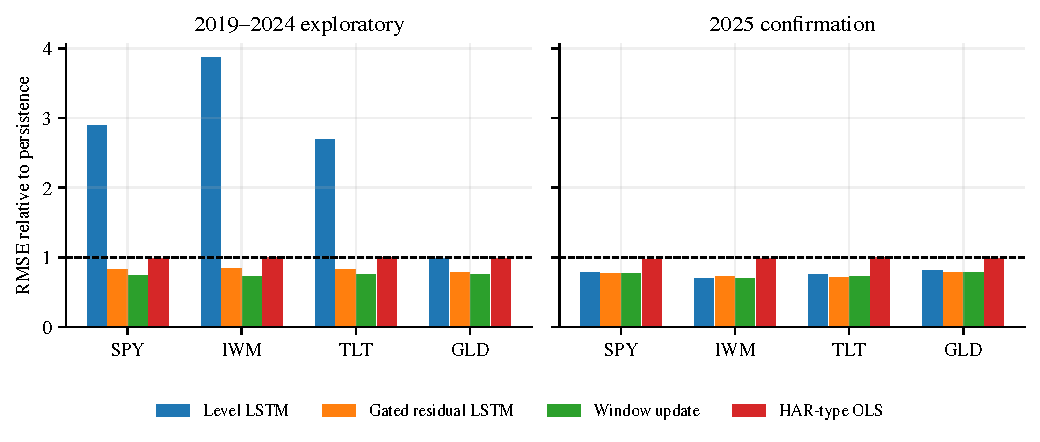
\includegraphics[width=\textwidth]{figures/study_forecast.pdf}
\caption{RMSE normalized by persistence, with the dashed line at one. Residual prediction removes much of the direct-level model's disadvantage. The window-update benchmark demonstrates that a substantial part of the gain concerns known rolling-window mechanics.}
\label{fig:forecast}
\end{figure*}

Table~\ref{tab:forecast} shows that the main neural comparison is materially different from a poorly performing level forecast. The gated residual model improves exploratory-period RMSE against persistence by 17.5\% for SPY, 16.0\% for IWM, 17.7\% for TLT, and 21.3\% for GLD. The corresponding confirmation improvements are approximately 22.6\%, 27.6\%, 28.5\%, and 21.8\%. Paired bootstrap intervals for residual-minus-persistence MSE lie below zero for all eight asset--period comparisons. These intervals are unadjusted descriptive summaries, not a claim of simultaneous or universal dominance.

The validation gate is one in 24 of the 28 asset--year fits and 0.75 in four. Thus the selected model does not achieve its result merely by reverting to persistence. The raw residual model is already substantially better than persistence; validation shrinkage makes relatively small changes. Reconstructing validation predictions from all saved residual checkpoints confirms that selected validation MSE never exceeds the persistence candidate's MSE.

The result is not evidence that neural complexity is essential. Equation~\eqref{eq:update} beats the selected residual model by RMSE for every asset in 2019--2024. Its residual-minus-update MSE intervals are positive. In 2025 the residual model is slightly better than the update forecast for TLT and GLD and slightly worse for SPY and IWM; all four corresponding difference intervals include zero. Figure~\ref{fig:forecast} therefore supports a narrower conclusion: an identity-anchored architecture is a fairer neural implementation, while simple conditional-moment structure remains highly competitive.

The level LSTM also performs considerably better in the confirmation year than in the exploratory aggregate, and its IWM RMSE is slightly lower than residual RMSE in 2025. This variation discourages a blanket claim that residual learning must outperform all level architectures. The main comparison includes EWMA, HAR-type OLS, and future five-day variation diagnostics in Appendix~\ref{app:forecast}, which distinguish predictability of the smoothed target from forecasting latent or forward risk.

\subsection{Calibration and predictive log scores}
\begin{table*}[t]
\centering\small
\caption{Parameters available at the start of 2025, estimated exclusively from past returns. $\theta$ is annual variance and $\mu$ annual physical drift. The final column is the standard deviation of total fitting log likelihood over five 4,096-particle evaluations; it is numerical variation, not a parameter standard error. Parameters are displayed to two significant figures.}
\label{tab:calibration}
\begin{tabular}{lrrrrrr}\toprule
ETF&$\kappa$&$\theta$&$\xi$&$\rho$&$\mu$&MC log-likelihood SD\\\midrule
SPY & 7.3 & 0.031 & 0.46 & -0.84 & 0.099 & 0.16 \\
IWM & 4.4 & 0.054 & 0.28 & -0.49 & 0.038 & 0.066 \\
TLT & 0.82 & 0.032 & 0.11 & -0.85 & -0.13 & 0.091 \\
GLD & 23 & 0.022 & 0.44 & 0.53 & 0.13 & 0.10
\\\bottomrule
\end{tabular}
\end{table*}
\begin{table*}[t]
\centering\small
\caption{Out-of-sample one-day return log scores from the latent-state filters. Higher is better. Difference is fitted minus the legacy fixed-parameter reference. Intervals are paired stationary-bootstrap summaries conditional on the fitted paths.}
\label{tab:logscores}
\begin{tabular}{llrrrr}\toprule
ETF&Period&Fitted&Fixed&Difference&95\% interval\\\midrule
SPY & 2019--24 & 3.2210 & 3.2256 & -0.0046 & [-0.0181, 0.0083] \\
SPY & 2025 & 3.2978 & 3.2803 & 0.0175 & [0.0007, 0.0360] \\
IWM & 2019--24 & 2.8120 & 2.8357 & -0.0237 & [-0.0469, -0.0050] \\
IWM & 2025 & 2.8924 & 2.9009 & -0.0085 & [-0.0250, 0.0075] \\
TLT & 2019--24 & 3.1533 & 3.1739 & -0.0206 & [-0.0832, 0.0173] \\
TLT & 2025 & 3.4925 & 3.4753 & 0.0172 & [-0.0005, 0.0352] \\
GLD & 2019--24 & 3.2730 & 3.2552 & 0.0179 & [-0.0181, 0.0444] \\
GLD & 2025 & 3.0122 & 2.9298 & 0.0824 & [0.0091, 0.1792]
\\\bottomrule
\end{tabular}
\end{table*}

Table~\ref{tab:calibration} reports asset-specific estimates available before 2025. Mean reversion ranges from about 0.82 for TLT to 23 for GLD, and return--variance correlation ranges from about $-0.85$ to $0.53$. Complete annual records appear in Appendix~\ref{app:parameters}. No retained fit lies within 1\% of a declared search boundary, but this does not establish parameter identification.

The fixed reference is a feasible candidate in the likelihood comparison. All 28 selected fitting scores exceed its score, so in-sample improvement is not an independent validation of the model. Out-of-sample results in Table~\ref{tab:logscores} are mixed: GLD has a higher mean fitted score in exploration, while SPY, IWM, and TLT have lower scores. In 2025 the fitted score is higher for SPY, TLT, and GLD and lower for IWM. The displayed confirmation intervals exclude zero for SPY and GLD, whereas those for TLT and IWM include zero. The exploratory IWM interval is below zero.

The reference uses common illustrative constants rather than a state-of-the-art likelihood estimator. All comparisons concern an approximate daily Euler model with bounded estimation and finite particles. They do not validate an exact continuous-time density or a market option surface.

\subsection{Fully invested portfolio outcomes}
\begin{table*}[t]
\centering\small\setlength{\tabcolsep}{4pt}
\caption{Broad model comparison with 2,000 scenarios at common unit gross ETF exposure. The higher-precision matched DRO comparison is in Table~\ref{tab:paired}. CAGR, daily loss ES, and maximum drawdown (MDD, positive magnitude) are percentages. SR is excess-return Sharpe against 3\% cash and $N_{\rm eff}$ the average effective ETF count. Calendar slices contain 1,508 and 247 daily returns. Holdings are carried into 2025 rather than restarted.}
\label{tab:portfolio}
\begin{tabular}{lrrrrrrrrrr}\toprule
&\multicolumn{5}{c}{2019--2024 exploratory}&\multicolumn{5}{c}{2025 confirmation}\\
\cmidrule(lr){2-6}\cmidrule(lr){7-11}
Strategy&CAGR&SR&ES&MDD&$N_{\rm eff}$&CAGR&SR&ES&MDD&$N_{\rm eff}$\\\midrule
Buy and hold & 10.36 & 0.627 & 1.83 & 25.16 & 3.85 & 31.57 & 1.946 & 1.95 & 11.32 & 3.50 \\
Equal weight & 9.98 & 0.605 & 1.77 & 24.65 & 4.00 & 26.80 & 1.796 & 1.72 & 10.49 & 4.00 \\
Minimum variance & 8.02 & 0.509 & 1.49 & 24.91 & 2.88 & 42.98 & 3.045 & 1.52 & 5.08 & 2.55 \\
Historical mean--CVaR & 4.36 & 0.164 & 2.20 & 32.77 & 1.78 & 61.25 & 2.675 & 2.53 & 8.24 & 1.21 \\
Fitted Heston / filter & 11.26 & 0.790 & 1.59 & 23.72 & 2.49 & 49.91 & 3.014 & 1.87 & 5.60 & 1.85 \\
Fitted Heston / persistence & 11.17 & 0.776 & 1.61 & 22.21 & 2.37 & 45.62 & 2.890 & 1.90 & 5.62 & 1.88 \\
Fitted Heston / residual & 11.04 & 0.766 & 1.60 & 22.55 & 2.37 & 45.83 & 2.926 & 1.87 & 5.62 & 1.88 \\
Fixed parameters / residual & 11.57 & 0.801 & 1.65 & 22.62 & 2.28 & 41.72 & 2.740 & 1.81 & 6.11 & 1.89 \\
Gaussian / residual & 11.62 & 0.796 & 1.67 & 22.21 & 2.20 & 41.28 & 2.710 & 1.82 & 6.00 & 1.85 \\
Fixed-radius DRO & 11.08 & 0.770 & 1.60 & 22.49 & 2.40 & 46.02 & 2.936 & 1.87 & 5.64 & 1.90 \\
Adaptive-radius DRO & 11.02 & 0.766 & 1.60 & 22.54 & 2.44 & 46.45 & 2.971 & 1.85 & 5.68 & 1.93
\\\bottomrule
\end{tabular}
\end{table*}
\begin{figure*}[t]
\centering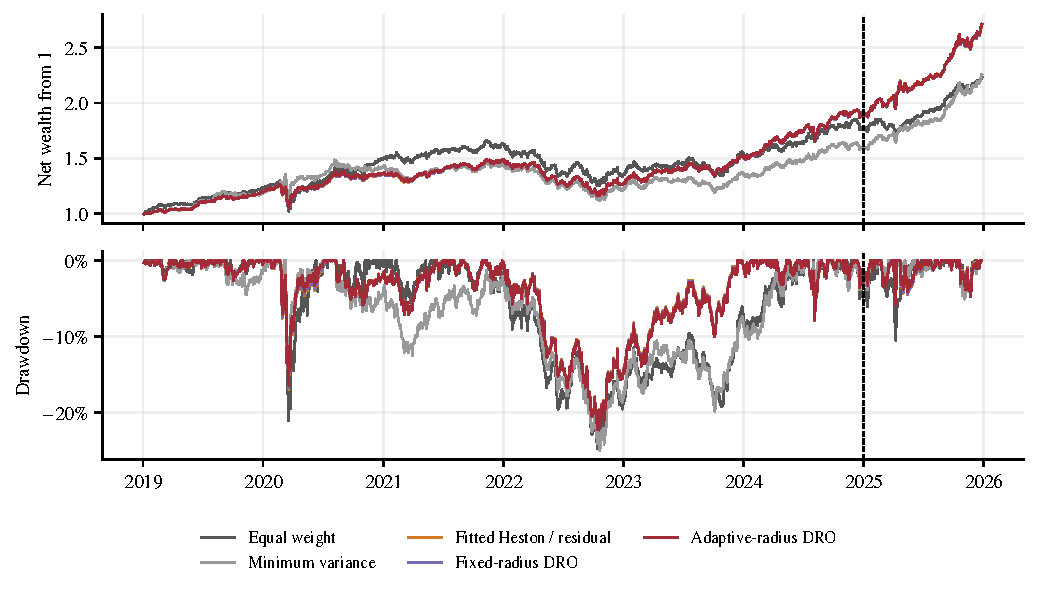
\includegraphics[width=\textwidth]{figures/study_wealth.pdf}
\caption{Net wealth and daily drawdown at equal total ETF exposure. Nominal and DRO curves use the primary 20,000-scenario seed; equal weight and minimum variance are historical-input references. The vertical line separates the exploratory sample from 2025 confirmation. A single favorable confirmation year does not establish persistent investment superiority.}
\label{fig:wealth}
\end{figure*}

The broad model comparison (Table~\ref{tab:portfolio}) is complemented by a matched higher-scenario experiment. The main economic assessment of robustness uses 20,000 scenarios and three independent seeds. All model parameters, expected returns, costs, and preferences are held common within that comparison; only the ambiguity radius differs. Holdings carry through the full historical path for each strategy and seed.

\begin{table*}[t]
\centering\small\setlength{\tabcolsep}{4pt}
\caption{Primary matched comparison at 20,000 scenarios, seed offset zero. Units match Table~\ref{tab:portfolio}; other seed outcomes are in Appendix~\ref{app:sensitivity}. The first seed was fixed in advance of this numerical comparison and was not chosen for its return.}
\label{tab:paired}
\begin{tabular}{lrrrrrrrrrr}\toprule
&\multicolumn{5}{c}{2019--2024 exploratory}&\multicolumn{5}{c}{2025 confirmation}\\
\cmidrule(lr){2-6}\cmidrule(lr){7-11}
Strategy&CAGR&SR&ES&MDD&$N_{\rm eff}$&CAGR&SR&ES&MDD&$N_{\rm eff}$\\\midrule
Fitted Heston / residual & 11.20 & 0.779 & 1.61 & 22.11 & 2.38 & 44.06 & 2.792 & 1.91 & 5.69 & 1.90 \\
Fixed-radius DRO & 11.18 & 0.779 & 1.60 & 22.19 & 2.42 & 44.39 & 2.810 & 1.91 & 5.74 & 1.92 \\
Adaptive-radius DRO & 11.21 & 0.783 & 1.60 & 22.25 & 2.46 & 44.59 & 2.849 & 1.88 & 5.82 & 1.95
\\\bottomrule
\end{tabular}
\end{table*}

In the primary 20,000-scenario path, nominal residual Heston earns 11.20\% exploratory CAGR and adaptive DRO 11.21\%. Their daily loss ES values are 1.606\% and 1.598\%. Adaptive DRO's maximum drawdown is 22.25\%, compared with 22.11\% nominally: smaller ES does not mean every realized risk measure improves. The corresponding confirmation CAGRs are 44.06\% and 44.59\%, with ES of 1.911\% and 1.881\%.

Every matched nominal and DRO rebalance in all three seeds holds at least two ETFs above the reporting threshold. Primary adaptive-DRO effective counts average 2.46 during exploration and 1.95 during confirmation, compared with nominal counts of 2.38 and 1.90. No per-asset cap forces these mixtures. Figure~\ref{fig:weights} shows primary-seed weights.

The 2,000-scenario model comparisons describe different scenario specifications rather than determine the main DRO conclusion. Filter-initialized Heston earns 49.91\% confirmation CAGR; historical mean--CVaR earns 61.25\% with greater concentration and tail loss. GLD's 63.7\% calendar return and the historical strategy's mean GLD weight of 90.2\% explain why that latter result is effectively a gold bet. The effective asset count is only 1.21. This is a favorable regime for concentrated gold exposure, not general confirmation of predictive superiority.

Fixed-parameter and Gaussian ablations slightly outperform the fitted residual specification by exploratory CAGR but trail it in confirmation. Estimation and stochastic-volatility dynamics are modeling choices whose economic value remains empirical. The residual forecast's incremental portfolio effect relative to persistence is also small. The broad 2,000-scenario and primary 20,000-scenario CAGRs differ because empirical tail approximations affect the optimizer; their difference motivates the matched higher-scenario comparison rather than a selection of the more favorable run.

\begin{figure*}[t]
\centering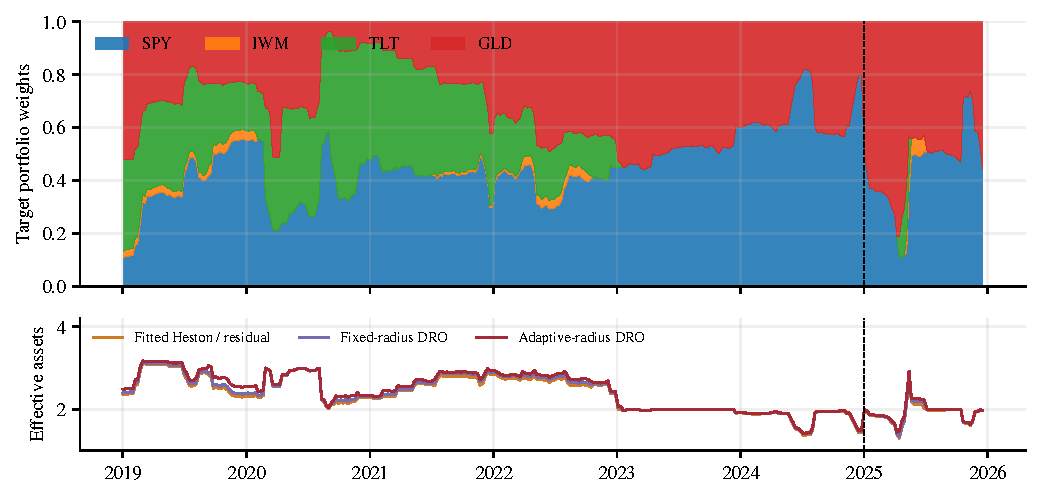
\includegraphics[width=\textwidth]{figures/study_weights.pdf}
\caption{Primary 20,000-scenario adaptive-DRO weights and effective ETF counts of matched model variants. Total ETF weight is one throughout. Allocations vary over time and hold multiple assets; the primary experiment cannot explain gains through an all-cash position.}
\label{fig:weights}
\end{figure*}

\subsection{Uncertainty, cash, and numerical scale}
\begin{table*}[t]
\centering\small\setlength{\tabcolsep}{4pt}
\caption{Robust allocation minus matched nominal residual Heston, at 20,000 scenarios and primary seed zero. Mean-return differences are annualized arithmetic percentage points. Daily ES differences are basis points, with negative values indicating lower tail loss. Intervals are unadjusted paired bootstrap percentiles.}
\label{tab:bootstrap}
\begin{tabular}{llrrrr}\toprule
Period&Robust strategy&Mean diff.&95\% interval&ES diff.&95\% interval\\\midrule
2019--24 & Fixed-radius DRO & -0.02 & [-0.11, 0.10] & -0.33 & [-0.81, 0.02] \\
2019--24 & Adaptive-radius DRO & 0.00 & [-0.23, 0.31] & -0.81 & [-2.04, 0.04] \\
2025 & Fixed-radius DRO & 0.23 & [-0.30, 0.82] & -0.03 & [-2.07, 2.45] \\
2025 & Adaptive-radius DRO & 0.35 & [-0.72, 1.46] & -3.02 & [-11.44, 4.14]
\\\bottomrule
\end{tabular}
\end{table*}
\begin{table*}[t]
\centering\small
\caption{Cash-enabled secondary experiment with 2,000 scenarios. CAGR and daily ES are percentages. Gross is mean risky ETF exposure in percent. The remaining wealth earns stylized 3\% annual cash interest. These portfolios solve a different mandate from the fully invested primary experiment.}
\label{tab:cash}
\begin{tabular}{lrrrrrr}\toprule
&\multicolumn{3}{c}{2019--2024 exploratory}&\multicolumn{3}{c}{2025 confirmation}\\
\cmidrule(lr){2-4}\cmidrule(lr){5-7}
Strategy&CAGR&ES&Gross&CAGR&ES&Gross\\\midrule
Fitted Heston / persistence & -0.03 & 1.20 & 38.75 & 5.49 & 0.13 & 3.82 \\
Fitted Heston / residual & -0.21 & 1.18 & 38.42 & 4.70 & 0.05 & 1.88 \\
Fixed-radius DRO & -0.48 & 1.16 & 37.03 & 3.71 & -0.01 & 0.35 \\
Adaptive-radius DRO & -0.54 & 1.12 & 35.19 & 3.16 & -0.01 & 0.08
\\\bottomrule
\end{tabular}
\end{table*}

Table~\ref{tab:bootstrap} shows no statistically reliable return advantage for either robust rule over matched nominal allocation. For adaptive DRO, the exploratory annualized arithmetic mean-return difference is approximately 0.003 percentage points, with interval $[-0.23,0.31]$. In confirmation the difference is 0.35 points, with interval $[-0.72,1.46]$. The primary-seed ES-difference intervals also include zero. These are descriptive, unadjusted intervals conditional on fitted paths.

The other two seeds preserve the direction of the confirmation return difference but do not establish significance. Across seeds, adaptive-minus-nominal mean-return differences range from about 0.08 to 0.35 annual percentage points in 2025; every corresponding interval includes zero. ES point differences are negative in both periods under all seeds. Two exploratory ES intervals exclude zero, whereas the primary interval and all confirmation intervals include zero. We do not select a seed because its interval is more favorable.

The conditional allocation experiment separates this statistical uncertainty from numerical resolution. At 2,000 scenarios, independent-seed adaptive-weight distances average about 0.022, exceeding within-seed robustness tilts of about 0.011--0.012. At 20,000 scenarios, average distances fall to 0.0053--0.0059, below tilts of 0.0128--0.0134 (Appendix~\ref{app:sensitivity}). The 95th-percentile distances remain larger than the mean tilt, so some dates remain more sensitive than average. Higher-scenario sampling resolves a small average allocation effect without supplying evidence of a reliable return improvement.

Cash-enabled results (Table~\ref{tab:cash}) concern a different mandate. Mean exploratory risky exposure is about 38.4\% for residual Heston and 35.2\% for adaptive DRO, with negative CAGRs despite smaller daily ES. In confirmation those risky exposures are about 1.88\% and 0.08\%, respectively. Lower risk largely reflects cash holdings. Negative displayed loss ES is possible when even the average worst-tail daily return is positive in a mostly cash portfolio.

Reference quantiles are imperfect. In the 2,000-scenario experiment, nominal residual-Heston and adaptive-DRO portfolios each breach their reference 5\% return quantile in 23 of 302 exploratory holding intervals (7.62\%) and one of 49 confirmation intervals (2.04\%). A robust objective adjustment does not produce a predictive VaR quantile or guarantee ambiguity-set membership. Radius, quadratic-risk, and fee sensitivities are descriptive grids reported in the appendix; no value is selected by confirmation performance.

\section{Discussion and limitations}
The study separates architecture, calibration, and allocation. An identity-anchored correction provides a fair neural comparison with persistence, but its target has overlapping observations. The window-update forecast explains much of the gain without a network. Claims about latent or forward variance require evidence beyond low error on a smoothed rolling window.

Fitting Heston parameters does not remove model risk. Predictive likelihood gains are mixed, despite tighter numerical searches and convergence of all refinement stages. The estimates remain conditional on a daily Euler likelihood, a Feller restriction, finite particles, and a bounded search. Resampling can produce irregular likelihood surfaces and weakly identified parameters. Displayed estimates have only two significant figures, and numerical likelihood variation is not parameter-estimation uncertainty.

With four risky assets and a quadratic risk term, allocations can change composition at fixed gross exposure. The cash-enabled comparison demonstrates that cash preference may nevertheless remain under estimated premia and the selected risk coefficient. A diversified decision space is necessary to study relative allocation, but it does not ensure attractive investment opportunities.

The 20,000-scenario experiment makes the numerical comparison more informative. Independent-seed allocation variation is smaller than the average robustness tilt, and the direction of the 2025 adaptive-minus-nominal return difference is stable across the three seeds. Statistical intervals nevertheless include zero. Numerical resolution and evidence of economic value are distinct questions. An absence of a statistically reliable gain under these settings is a substantive result, rather than a claim that every robustness effect is hidden by the simulator.

The 2025 confirmation sample is unusually favorable to gold. GLD's adjusted-close calendar return is 63.7\%, compared with 17.7\% for SPY, 12.7\% for IWM, and 4.2\% for TLT. The historical mean--CVaR benchmark averages about 90\% GLD weight and an effective asset count of 1.21. Its roughly 61\% annualized CAGR is largely a concentrated gold position. It is not broad evidence that its risk model forecasts well. Calendar close-to-close asset returns and the 247-day adjusted-open portfolio slice have different boundaries, so these figures are explanatory context rather than an exact return attribution.

Other limitations remain material. SPY and IWM share substantial equity exposure, and four ETFs cannot represent all market opportunities. Dependence uses shrunk return correlation and a restricted shock construction. Neural rolling-volatility forecasts approximate an instantaneous variance state. Drifts are noisy and do not establish return predictability. Adjusted-open execution assumes immediate fills after observing the mark; spreads, slippage, taxes, and delay are omitted. The linear fee proxy differs from exact compounded deductions by interaction terms.

The exploratory sample motivated the design, and confirmation covers only one historical year. Bootstrap intervals assume a useful degree of stationarity, do not refit models, and are unadjusted for multiple comparisons. Exact replication also requires access to matching third-party inputs. Public code, hashes, model records, and summaries make the computational procedure inspectable, but they do not grant data rights or ensure that providers retain an unchanged historical snapshot.

Future work can use intraday measures or direct forward targets, assess parameter identification with more accurate likelihoods, test other universes and confirmation periods, and calibrate transport radii against held-out distributional errors.

\section{Conclusion}
This selective review combines established DRO methods with residual volatility forecasting, fitted physical Heston dynamics, and convex multi-asset allocation. Persistence is explicit in the neural architecture, structural parameters use historically available returns, and fixed total ETF exposure separates composition from cash-based de-risking.

Residual forecasting improves on persistence while a simple window-update model remains competitive. Heston likelihood gains are mixed. Higher-scenario paired allocation runs resolve a small robustness-induced change in weights, but do not establish a statistically reliable return advantage over matched nominal allocation. Strong 2025 CAGRs must be interpreted alongside a gold rally and concentrated gold exposure. The public computational record supports a reproducible case study of these established components, with conditional data access and restrained performance claims.

\section*{Code and data availability}
Code, configuration, 168 trained network checkpoints, 28 annual parameter-fit records, aggregate results, input hashes, and figure/table scripts are available in the versioned public GitHub release \cite{repository}:\par
\noindent{\footnotesize\url{https://github.com/Sheehan007/Distributionally-Robust-Optimization/releases/tag/v1.0.0}}\par
Provider observations, raw API responses, and date-by-date market and portfolio caches are excluded from public artifacts. The release documents Yahoo's and Cboe's terms and provides a downloader requiring explicit acknowledgment of those terms. Exact numerical replication is conditional on appropriate access and matching canonical input hashes. A provider-history change produces a new-data evaluation, not an exact replication of the reported snapshot.

\section*{Author and tool disclosure}
Sheehan Mathur is the sole author. Anthropic Claude assisted with Table~\ref{tab:families} and parts of the literature-review text. OpenAI Codex assisted with implementation audits, experiment development and execution, drafting, reference checking, and typesetting. The author is responsible for the final scientific interpretation and submission.

\FloatBarrier
\appendix
\section{Transport identity and curvature}
\label{app:transport}
For fixed $w$, the loss $\ell_w(r)=-w^\top r$ is $\lVert w\rVert_2$-Lipschitz. The positive-part CVaR representation gives the upper bound
\begin{equation}
\CVaR^Q_\alpha(\ell_w)\leq
\CVaR^{\widehat P_N}_\alpha(\ell_w)+\frac{\epsilon\lVert w\rVert_2}{1-\alpha}
\end{equation}
whenever $W_1(Q,\widehat P_N)\leq\epsilon$. To attain it on unrestricted support, select exactly $q=1-\alpha$ mass from the largest nominal losses, splitting boundary atoms if necessary. For $w\ne0$, move this mass in return space by
\begin{equation}
-\frac{\epsilon}{q}\frac{w}{\lVert w\rVert_2}.
\end{equation}
The transport plan costs $\epsilon$, increases each selected loss by $\epsilon\lVert w\rVert_2/q$, and preserves its position in the upper tail. Its tail average attains the upper bound. For $w=0$ both sides vanish. This specializes established Wasserstein risk reformulations \cite{esfahani,kuhntutorial}; it is not a new theorem. Atom splitting also explains why empirical ES averages fractional boundary mass when $Nq$ is noninteger.

Equation~\eqref{eq:allocation} retains nominal mean return. If one instead robustifies mean minus $\gamma$ times CVaR under the \emph{same} adverse law, this transport also lowers the mean by $\epsilon\lVert w\rVert_2$. The penalty becomes $\epsilon\lVert w\rVert_2[1+\gamma/(1-\alpha)]$. That alternative is not the implemented objective. Support constraints require a new derivation.

The covariance ridge makes $\Omega_t$ positive definite for the nondegenerate scenario samples used here. For $\lambda>0$, $-\lambda w^\top\Omega_t w/2$ is strictly concave. The remaining terms in \eqref{eq:allocation} are concave, so the objective is strictly concave on the convex feasible set and has a unique maximizer. Uniqueness does not imply strictly positive components. Actual multi-asset holdings are an empirical result, reported separately from this mathematical property.

\section{Additional forecast diagnostics}
\label{app:forecast}
\begin{table*}[t]
\centering\small\setlength{\tabcolsep}{5pt}
\caption{Additional forecast diagnostics. MAE concerns log next-day rolling volatility. F-QLIKE concerns annualized future five-day squared-return variation on nonoverlapping target windows. Lower is better. This separate future target was not the training objective and is not observed latent variance.}
\label{tab:additional_forecast}
\begin{tabular}{llrrrrrr}\toprule
& &\multicolumn{2}{c}{Persistence}&\multicolumn{2}{c}{Window update}&\multicolumn{2}{c}{Gated residual}\\
\cmidrule(lr){3-4}\cmidrule(lr){5-6}\cmidrule(lr){7-8}
ETF&Period&MAE&F-QLIKE&MAE&F-QLIKE&MAE&F-QLIKE\\\midrule
SPY & 2019--24 & 0.0386 & 0.6032 & 0.0281 & 0.5976 & 0.0349 & 0.5565 \\
SPY & 2025 & 0.0414 & 0.7706 & 0.0289 & 0.7563 & 0.0334 & 0.7176 \\
IWM & 2019--24 & 0.0355 & 0.4593 & 0.0259 & 0.4637 & 0.0305 & 0.4475 \\
IWM & 2025 & 0.0370 & 0.4767 & 0.0265 & 0.4677 & 0.0288 & 0.4511 \\
TLT & 2019--24 & 0.0333 & 0.3682 & 0.0250 & 0.3849 & 0.0286 & 0.3673 \\
TLT & 2025 & 0.0358 & 0.2525 & 0.0245 & 0.2580 & 0.0262 & 0.2527 \\
GLD & 2019--24 & 0.0374 & 0.4780 & 0.0281 & 0.4853 & 0.0317 & 0.4698 \\
GLD & 2025 & 0.0416 & 0.6057 & 0.0293 & 0.5845 & 0.0332 & 0.5482
\\\bottomrule
\end{tabular}
\end{table*}
Table~\ref{tab:additional_forecast} distinguishes the smoothed target from future variation. Residual forecasts have lower displayed future QLIKE than persistence in seven of eight asset--period comparisons; TLT in 2025 is slightly worse. These point estimates do not supply an inference about true latent variance. All model-level RMSE, MAE, rolling-proxy QLIKE, annual seed errors, and paired loss-difference intervals are retained in the companion CSV files, including the EWMA and HAR-type comparators.

\section{Annual parameter estimates}
\label{app:parameters}
\begin{table*}[t]
\centering\footnotesize\setlength{\tabcolsep}{5pt}
\caption{All annual physical-model fits, displayed to two significant figures. LL gain is fitted minus fixed-reference total log likelihood on the same 756 fitting returns. MC SD is fitted likelihood variation across five 4,096-particle seeds. Neither is a parameter uncertainty interval. Data-dependent starting values, the fixed reference, and fitted candidates are compared by training likelihood only.}
\label{tab:all_parameters}
\begin{tabular}{llrrrrrr}\toprule
ETF&Test year&$\kappa$&$\theta$&$\xi$&$\rho$&LL gain&MC SD\\\midrule
SPY & 2019 & 11 & 0.015 & 0.46 & -0.54 & 12.31 & 0.34 \\
SPY & 2020 & 9.9 & 0.014 & 0.44 & -0.71 & 16.77 & 0.35 \\
SPY & 2021 & 6.4 & 0.056 & 0.72 & -0.60 & 31.63 & 0.21 \\
SPY & 2022 & 10 & 0.032 & 0.71 & -0.67 & 37.09 & 0.75 \\
SPY & 2023 & 7.7 & 0.053 & 0.78 & -0.74 & 31.05 & 0.41 \\
SPY & 2024 & 8.6 & 0.031 & 0.55 & -0.78 & 5.29 & 0.21 \\
SPY & 2025 & 7.3 & 0.031 & 0.46 & -0.84 & 3.55 & 0.16 \\
IWM & 2019 & 8.2 & 0.027 & 0.41 & -0.71 & 1.16 & 0.12 \\
IWM & 2020 & 11 & 0.022 & 0.44 & -0.78 & 6.34 & 0.18 \\
IWM & 2021 & 4.9 & 0.058 & 0.68 & -0.62 & 23.88 & 0.24 \\
IWM & 2022 & 5.4 & 0.070 & 0.82 & -0.67 & 30.82 & 0.56 \\
IWM & 2023 & 8.0 & 0.093 & 0.93 & -0.70 & 32.26 & 0.32 \\
IWM & 2024 & 6.5 & 0.056 & 0.36 & -0.58 & 3.37 & 0.14 \\
IWM & 2025 & 4.4 & 0.054 & 0.28 & -0.49 & 3.51 & 0.066 \\
TLT & 2019 & 0.63 & 0.011 & 0.046 & 0.57 & 36.98 & 0.079 \\
TLT & 2020 & 0.73 & 0.012 & 0.071 & 0.79 & 46.83 & 0.15 \\
TLT & 2021 & 11 & 0.019 & 0.43 & 0.14 & 45.02 & 0.47 \\
TLT & 2022 & 14 & 0.023 & 0.51 & 0.079 & 38.29 & 1.2 \\
TLT & 2023 & 9.2 & 0.039 & 0.53 & -0.046 & 26.27 & 0.35 \\
TLT & 2024 & 1.3 & 0.037 & 0.12 & -0.50 & 6.43 & 0.15 \\
TLT & 2025 & 0.82 & 0.032 & 0.11 & -0.85 & 10.34 & 0.091 \\
GLD & 2019 & 2.1 & 0.013 & 0.096 & 0.31 & 32.23 & 0.13 \\
GLD & 2020 & 11 & 0.011 & 0.18 & 0.50 & 45.26 & 0.086 \\
GLD & 2021 & 16 & 0.018 & 0.51 & 0.25 & 48.26 & 0.23 \\
GLD & 2022 & 19 & 0.023 & 0.71 & 0.14 & 45.86 & 0.32 \\
GLD & 2023 & 25 & 0.026 & 0.69 & 0.038 & 38.94 & 0.18 \\
GLD & 2024 & 27 & 0.020 & 0.51 & 0.14 & 27.61 & 0.15 \\
GLD & 2025 & 23 & 0.022 & 0.44 & 0.53 & 33.13 & 0.10
\\\bottomrule
\end{tabular}
\end{table*}
\begin{figure*}[t]
\centering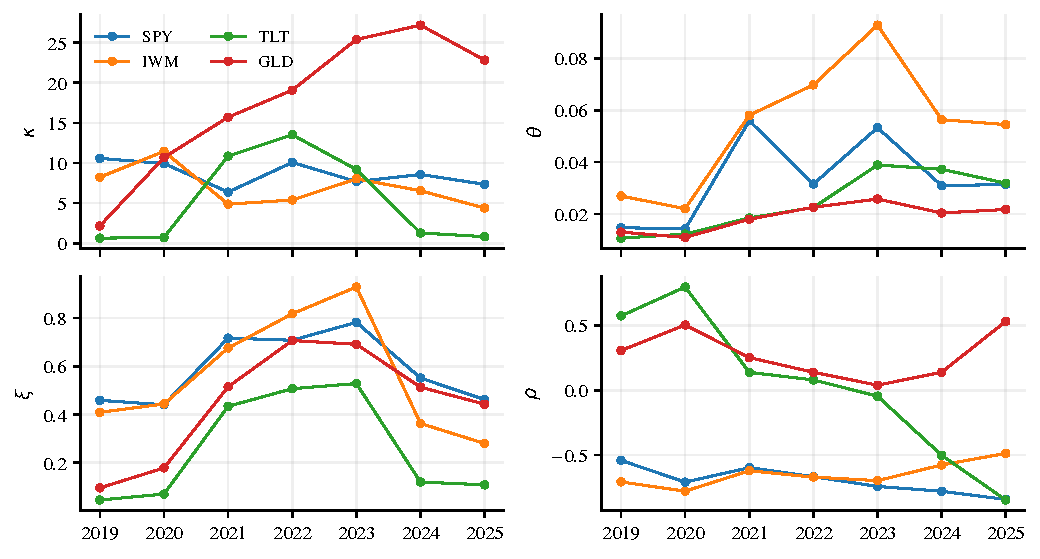
\includegraphics[width=\textwidth]{figures/study_calibration.pdf}
\caption{Annual asset-specific estimates available before each evaluation year. Changes reflect rolling historical samples and approximate bounded estimation, rather than parameter changes inferred from the later evaluation outcomes.}
\label{fig:parameters}
\end{figure*}
Table~\ref{tab:all_parameters} and Figure~\ref{fig:parameters} make the annual estimates explicit. All refinement stages meet their numerical stopping condition. Five selected fits retain an archived likelihood-based start when its five-seed checking score exceeds the other candidates. Thus tighter searches do not imply that every selected coordinate has moved away from a line-search trial value. Finite-particle irregularity and identification limitations remain, and two significant figures are used throughout the parameter tables. Full computational values, starts, search statuses, likelihood evaluations, Feller gaps, and causal fit dates are archived.

\section{Sensitivity and simulation checks}
\label{app:sensitivity}
\begin{table*}[t]
\centering\small\setlength{\tabcolsep}{5pt}
\caption{Declared 2,000-scenario sensitivities, evaluated on 2025 calendar returns after recomputing complete paths from 2019. Radius values are vector simple-return distances; costs are fractions of risky turnover. CAGR and daily ES are percentages. Other coefficients retain their primary settings.}
\label{tab:sensitivity}
\begin{tabular}{lllr rr}\toprule
Setting&Value&Strategy&CAGR&ES&$N_{\rm eff}$\\\midrule
epsilon & 0 & Fixed-radius DRO & 45.83 & 1.87 & 1.88 \\
epsilon & 5e-05 & Fixed-radius DRO & 45.90 & 1.87 & 1.89 \\
epsilon & 0.0001 & Fixed-radius DRO & 46.02 & 1.87 & 1.90 \\
epsilon & 0.00025 & Fixed-radius DRO & 46.62 & 1.87 & 1.92 \\
epsilon & 0.0005 & Fixed-radius DRO & 46.44 & 1.88 & 1.95 \\
lambda & 0 & Fixed-radius DRO & 47.88 & 2.05 & 1.80 \\
lambda & 1 & Fixed-radius DRO & 46.99 & 2.01 & 1.83 \\
lambda & 4 & Fixed-radius DRO & 46.02 & 1.87 & 1.90 \\
lambda & 10 & Fixed-radius DRO & 43.37 & 1.74 & 1.98 \\
cost & 0 & Fitted Heston / residual & 54.27 & 1.72 & 1.82 \\
cost & 0 & Fixed-radius DRO & 53.67 & 1.71 & 1.83 \\
cost & 0 & Adaptive-radius DRO & 53.06 & 1.69 & 1.85 \\
cost & 0.0007 & Fitted Heston / residual & 45.83 & 1.87 & 1.88 \\
cost & 0.0007 & Fixed-radius DRO & 46.02 & 1.87 & 1.90 \\
cost & 0.0007 & Adaptive-radius DRO & 46.45 & 1.85 & 1.93 \\
cost & 0.0014 & Fitted Heston / residual & 38.29 & 2.01 & 1.93 \\
cost & 0.0014 & Fixed-radius DRO & 38.38 & 2.00 & 1.94 \\
cost & 0.0014 & Adaptive-radius DRO & 38.58 & 1.97 & 1.97
\\\bottomrule
\end{tabular}
\end{table*}
\begin{table*}[t]
\centering\small\setlength{\tabcolsep}{5pt}
\caption{Conditional 2025 allocation checks at 2,000 and 20,000 scenarios under independent draws. Distance is adaptive-DRO weight $L^1$ distance from seed zero at the same scenario count; tilt is its distance from matched nominal allocation under the same draws. Every check uses common pretrade weights reconstructed from the primary 20,000-scenario nominal path. These are allocation diagnostics, separate from the full backtests.}
\label{tab:monte_carlo}
\begin{tabular}{rrrrr}\toprule
Scenarios&Seed offset&Mean distance&95th percentile&Mean robustness tilt\\\midrule
2000 & 0 & 0.0000 & 0.0000 & 0.0112 \\
2000 & 10000 & 0.0224 & 0.1225 & 0.0119 \\
2000 & 20000 & 0.0225 & 0.1126 & 0.0123 \\
20000 & 0 & 0.0000 & 0.0000 & 0.0128 \\
20000 & 10000 & 0.0053 & 0.0236 & 0.0134 \\
20000 & 20000 & 0.0059 & 0.0285 & 0.0130
\\\bottomrule
\end{tabular}
\end{table*}
The sensitivity grid is descriptive; it is not a search for a preferred test-period coefficient. Higher fees change the optimizer's trading decisions as well as realized deductions. The $\lambda=0$ row removes the quadratic term while retaining multivariate CVaR, costs, and the fixed-radius norm penalty. Such a multivariate problem is not subject to the original single-exposure endpoint argument.

At 2,000 scenarios, mean independent-seed allocation distances of about 0.022 exceed robustness tilts near 0.012. At 20,000 scenarios, mean distances decrease to about 0.005--0.006, while tilts remain near 0.013. Both counts use their own first-seed reference and identical pretrade weights, so this reduction is not measured against a noisy lower-count reference. Some dates remain sensitive, as the 95th-percentile distances show. Three seeds characterize numerical variation rather than establish an asymptotic convergence rate.

\begin{table*}[t]
\centering\small\setlength{\tabcolsep}{6pt}
\caption{Full-path 20,000-scenario seed sensitivity. CAGRs and annualized arithmetic mean-return differences are percentages; ES differences are daily basis points. Every difference is adaptive DRO minus matched nominal allocation. Complete paired intervals for every seed are public.}
\label{tab:paired_seeds}
\begin{tabular}{rlrrrr}\toprule
Seed offset&Period&Nominal CAGR&Adaptive CAGR&Mean diff.&ES diff.\\\midrule
0 & 2019--24 & 11.20 & 11.21 & 0.003 & -0.81 \\
0 & 2025 & 44.06 & 44.59 & 0.353 & -3.02 \\
10000 & 2019--24 & 11.16 & 11.18 & 0.013 & -0.86 \\
10000 & 2025 & 43.89 & 44.02 & 0.075 & -3.22 \\
20000 & 2019--24 & 11.22 & 11.27 & 0.040 & -0.97 \\
20000 & 2025 & 43.59 & 43.94 & 0.235 & -2.39
\\\bottomrule
\end{tabular}
\end{table*}
The three full backtests use independent simulator draws for the whole 2019--2025 path. No holdings restart at the confirmation boundary. Table~\ref{tab:paired_seeds} displays their variation without choosing the most favorable seed. Mean-return intervals include zero in every comparison.

\section{Reproduction and validation}
\label{app:reproduction}
The versioned public release contains executable code, a design protocol, input hashes and source URLs, trained model checkpoints, annual fit records, and aggregate diagnostics. Provider observations and date-by-date experimental caches are excluded. A reader with appropriate data access can download local inputs, verify their canonical hashes, reconstruct neural predictions with \texttt{forecast.py --reuse-checkpoints}, rebuild latent-state paths with \texttt{calibrate.py}, and run \texttt{portfolio.py}, \texttt{paired\_accuracy.py}, \texttt{analyze.py}, \texttt{analyze\_accuracy.py}, \texttt{extra\_checks.py}, and \texttt{paper\_assets.py}. The README distinguishes exact matching-input replication from a current-provider-data rerun. Public summaries suffice to regenerate the numerical tables and the forecast/parameter figures; wealth and allocation figures require regenerated local paths.

Ten mathematical and timing tests pass. Nine cover the persistence identity, fractional-mass ES versus an independent linear program, explicit multivariate tail transport, a known quadratic portfolio solution, CVaR versus an independent program, deterministic-variance Gaussian filtering, leverage-conditioned variance means, causal dates, and portfolio feasibility/common holding intervals. A tenth compares the tail-separation solver with the full empirical conic epigraph, including fractional tail mass and cash-enabled cases. Checkpoint replay reconstructs all saved forecasts to numerical precision, and all 28 validation gates are independently checked.

The primary paired experiment contains 3,159 portfolio solves. Sixty-two final statuses are \texttt{optimal\_inaccurate}; every solution nevertheless passes the recorded primal feasibility and full-scenario tail-separation checks, with maximum violations below $2\times10^{-10}$ and tail-objective underestimation below $10^{-10}$. These diagnostics do not turn an approximate solver status into a formal exact-arithmetic certificate. As an additional check, eight independent full-epigraph solves on four fixed schedule positions with 20,000 scenarios differ in objective by at most $1.2\times10^{-10}$ and in weight $L^1$ distance by at most $1.1\times10^{-4}$. The dates and differences are public. These checks validate computational behavior, not market generalization.

\FloatBarrier
\balance
\bibliographystyle{unsrt}
\begingroup\small\raggedright\bibliography{references}\endgroup
\end{document}
